\begin{tikzpicture}
    \node[anchor=south west,inner sep=0] (image) at (0,0) {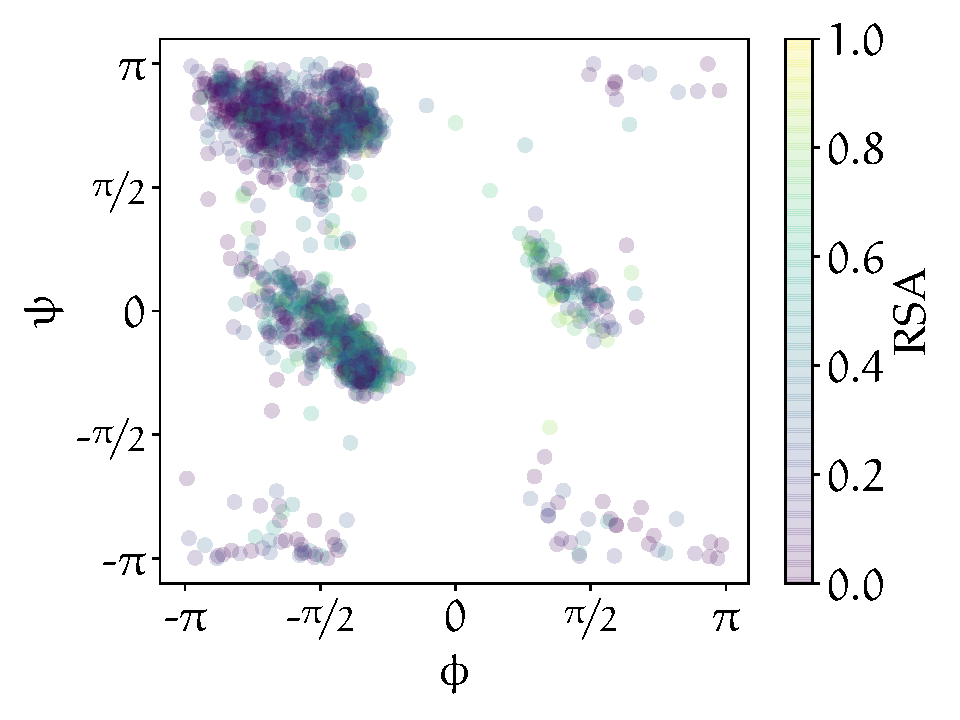
\includegraphics[width=0.9\columnwidth]{machine_learning/figures/transfer_learning}};
    \begin{scope}[x={(image.south east)},y={(image.north west)}]
    	\coordinate (a1) at (0.6,0.6);
    	\coordinate (a2) at (0.4,0.45);
    	\coordinate (al) at (0.5, 0.3);
    	\coordinate (bl) at (0.52, 0.88);
    	\coordinate (b) at (0.39, 0.88);
    	\draw[->, >=stealth, Maroon, thick] ( $ (al) !0.15! (a1)$ ) -- ( $ (al) !0.75! (a1)$ ) node {};
    	\draw[->, >=stealth, Maroon, thick] ( $ (al) !0.25! (a2)$ ) -- ( $ (al) !0.75! (a2)$ ) node {};
    	\node[Maroon] (O) at (al) {\Large $\alpha$};
    	\draw[->, >=stealth, Maroon, thick] ( $ (bl) !0.25! (b)$ ) -- ( $ (bl) !0.75! (b)$ ) node {};
    	\node[Maroon] (O) at (bl) {\Large $\beta$};

        %\draw[help lines,xstep=.1,ystep=.1] (0,0) grid (1,1);
        %\foreach \x in {0,1,...,9} { \node [anchor=north] at (\x/10,0) {0.\x}; }
        %\foreach \y in {0,1,...,9} { \node [anchor=east] at (0,\y/10) {0.\y}; }
    \end{scope}
\end{tikzpicture}
